\chapter{評価実験}

\label{chap:evaluation}

\section{実験環境}
	\subsection{データセット生成}
		感性語の抽出を行うにあたり,感情表現辞典に掲載された情報を活用する.
		感情表現辞典に収録されている単語と熟語の合計2278語のうち,
		MeCabで分かち書きを行うことで複数単語に別れてしまうものを除くと,
		1245語となる.
		なお,MeCabの辞書にはipadicを用いた.
		本実験におけるデータセット生成では,これらを感性語とする.

		データセット生成のためのテキストデータには
		Wikipedia\cite{wikipedia}のテキストに前処理を施した状態で公開されている
		Wiki-40B\cite{wiki-40b}データセットの日本語版を用いる.
		1文ずつに分割し,感性語を含む文章のみを抽出した.
		それぞれの文章の数は以下の表\ref{table:wiki40b_sentence}の通りである.
		\begin{table}[H]
			\centering
			\caption{wiki-40bデータセットから得られる文章の数}
			\label{table:wiki40b_sentence}
			\begin{tabular}{cccc}
				\hline
				& Train & Val & Test \\
				\hline \hline
				全文章 & 12,330,278 & 677,757 & 678,490 \\
				感性語を含む文章 & 2,337,909 & 128,126 & 128,698 \\
				\hline
			\end{tabular}
		\end{table}
		% $Train/Val/Test=12,330,278/677,757/678,490$となった.
		% これらのうち,感性語を含む文は
		% $Train/Val/Test=2,337,909/128,126/128,698$となった.
		本実験では,ウィンドウサイズ$W=3$とし,感性語の周辺単語を収集した.
		このBERTが出力した分散表現と感情ベクトルがペアになった
		データセットのサイズは,
		% $Train/Val/Test=20,154,529/1,104,904/1,108,482$
		% となった.
		以下の表\ref{table:bert_to_emo_size}の通りである.
		\begin{table}[H]
			\centering
			\caption{作成したデータセットのサイズ}
			\label{table:bert_to_emo_size}
			\begin{tabular}{ccc}
				\hline
				Train & Val & Test \\
				\hline \hline
				20,154,529 & 1,104,904 & 1,108,482 \\
				\hline
			\end{tabular}
		\end{table}
		なお,用いたBERTモデルはHugging Face\cite{huggingface}で東北大学が公開している
		cl-tohoku/bert-base-japanese-whole-word-masking\cite{cl-tohoku}である.

	\subsection{ニューラルネットワークの学習条件}
		入力が768次元の単語分散表現で,出力が10次元の感情ベクトルとなる.
		本実験では図\ref{fig:network}で示すような,中間層を400次元とした
		非常にシンプルな3層のニューラルネットワークを構築し,
		生成したデータセットを用いて学習を行った.
				
		損失関数は最小二乗誤差とし,Adamにより学習率$1\times10^{-3}$で最適化を行った.
		エポック数については,Early Stoppingで5回以上validation lossが更新
		されなかった段階で学習を終了させた.
		
	\subsection{比較手法}
		本手法と比較するためのベースライン手法として,BERT Layerを通す前の
		Embedding Layerによる分散表現をネットワークの入力とした場合を設定する.
		BERT Layerを通すことにより,Transformerによる周りの単語の影響を加味することになる.
		今回設定したベースラインではEmbedding Layerによる
		分散表現を利用することで周辺単語の影響が含まれないことになる.
		また、感性語の周辺単語に与える感情ベクトルについて
		距離に応じた重み付けを行うことによる効果を確認するため,
		重み付けを行うBERT+weight,行わないBERTに分けて実験を行う.

\section{感情ベクトルの生成例}
	入力文に対する各単語の感情ベクトル出力例を以下に示す.
	\subsection{「仕事は人生を豊かにしてくれる.」に対する出力}
		\begin{figure}[H]
			\begin{tabular}{cc}
				\begin{minipage}[t]{0.45\hsize}
					\centering
					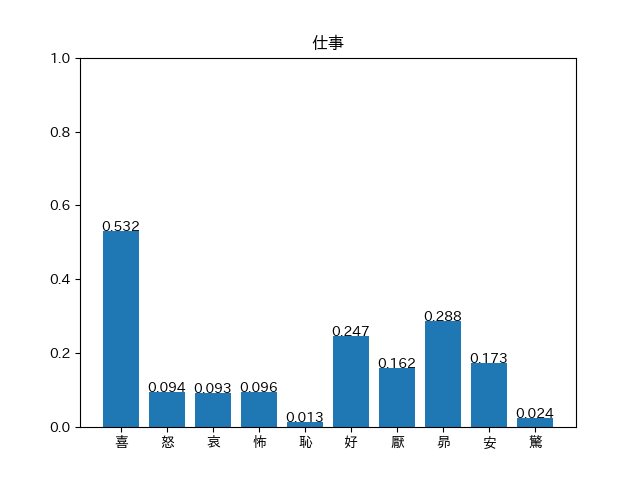
\includegraphics[keepaspectratio, scale=0.45]{./figure/output/Q01/001.png}
					\subcaption{「仕事」に対する感情ベクトル}
				\end{minipage} &
				\begin{minipage}[t]{0.45\hsize}
					\centering
					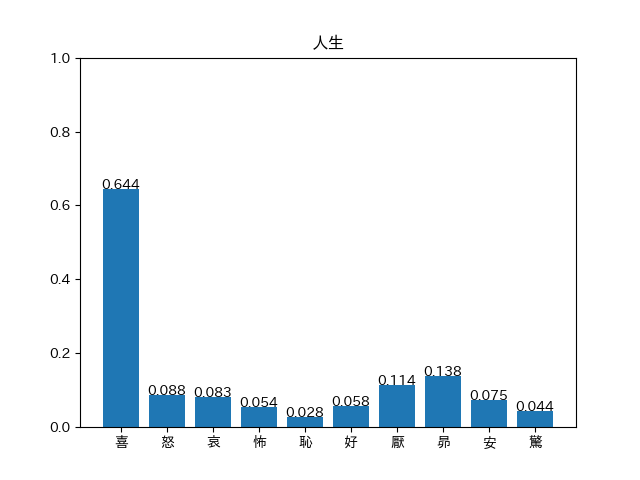
\includegraphics[keepaspectratio, scale=0.45]{./figure/output/Q01/002.png}
					\subcaption{「人生」に対する感情ベクトル}
				\end{minipage} \\
				\begin{minipage}[t]{0.45\hsize}
					\centering
					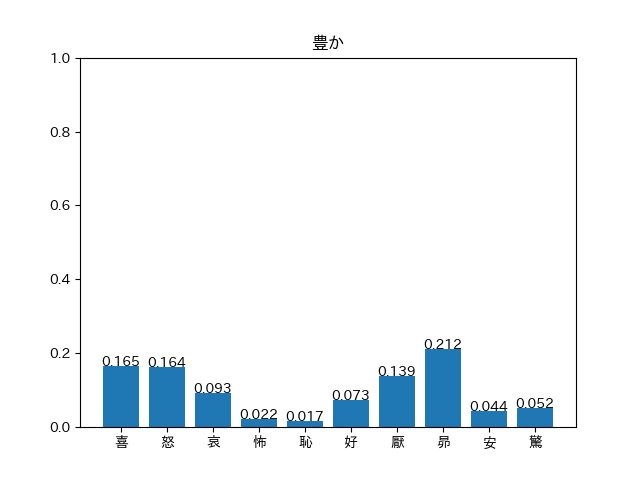
\includegraphics[keepaspectratio, scale=0.45]{./figure/output/Q01/003.png}
					\subcaption{「豊か」に対する感情ベクトル}
				\end{minipage} &
				\begin{minipage}[t]{0.45\hsize}
					\centering
					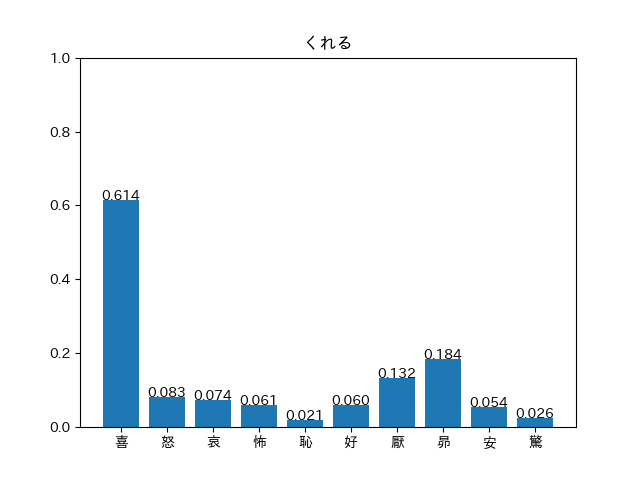
\includegraphics[keepaspectratio, scale=0.45]{./figure/output/Q01/004.png}
					\subcaption{「くれる」に対する感情ベクトル}
				\end{minipage} \\
			\end{tabular}
			\caption{「仕事は人生を豊かにしてくれる.」に対する各単語の感情ベクトル}
			\label{fig:output_ex01}
		\end{figure}

	\subsection{「仕事は面倒だし、疲れるから嫌だ。」に対する出力}
		\begin{figure}[H]
			\begin{tabular}{cc}
				\begin{minipage}[t]{0.45\hsize}
					\centering
					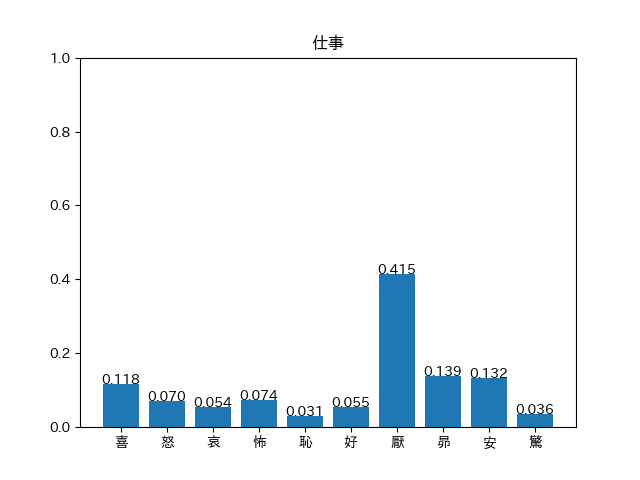
\includegraphics[keepaspectratio, scale=0.45]{./figure/output/Q02/001.png}
					\subcaption{「仕事」に対する感情ベクトル}
				\end{minipage} &
				\begin{minipage}[t]{0.45\hsize}
					\centering
					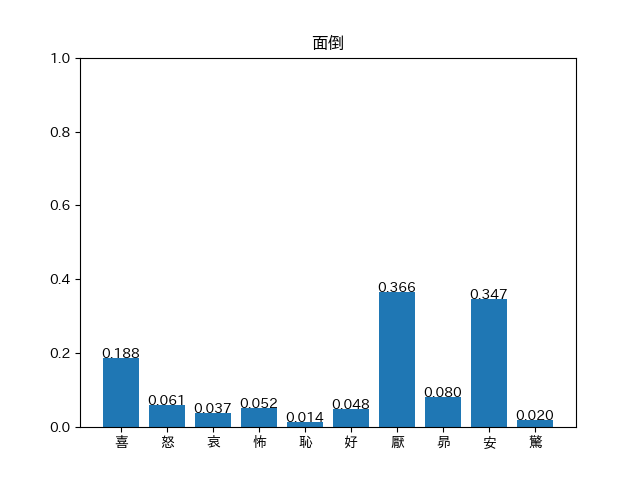
\includegraphics[keepaspectratio, scale=0.45]{./figure/output/Q02/002.png}
					\subcaption{「面倒」に対する感情ベクトル}
				\end{minipage} \\
				\begin{minipage}[t]{0.45\hsize}
					\centering
					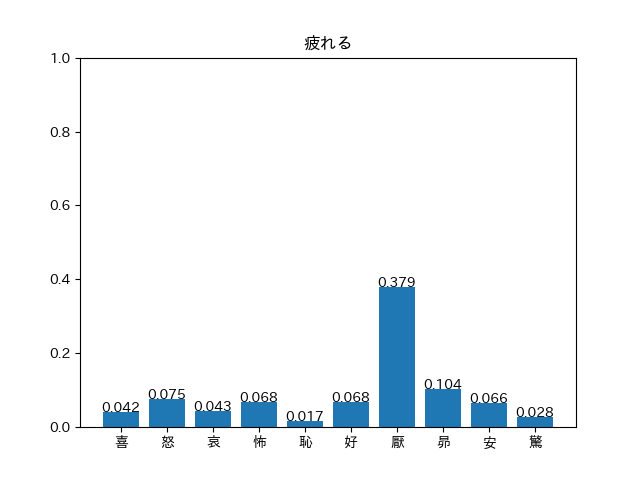
\includegraphics[keepaspectratio, scale=0.45]{./figure/output/Q02/003.png}
					\subcaption{「疲れる」に対する感情ベクトル}
				\end{minipage} &
				\begin{minipage}[t]{0.45\hsize}
					\centering
					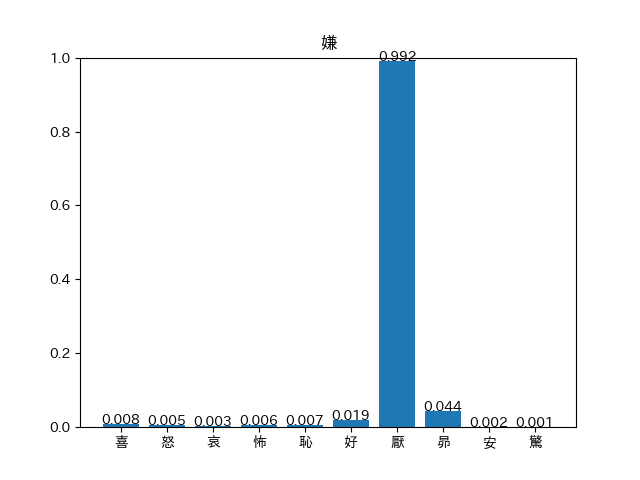
\includegraphics[keepaspectratio, scale=0.45]{./figure/output/Q02/004.png}
					\subcaption{「嫌」に対する感情ベクトル}
				\end{minipage} \\
			\end{tabular}
			\caption{「仕事は面倒だし、疲れるから嫌だ.」に対する各単語の感情ベクトル}
			\label{fig:output_ex02}
		\end{figure}

		図\ref{fig:output_ex01}ではポジティブな文脈で「仕事」という単語を用いているのに対し,
		図\ref{fig:output_ex02}ではネガティブな文脈で「仕事」という単語を用いている.
		それぞれの「仕事」に対する感情ベクトルを比較すると,
		文脈に応じてその出力が変化していることがわかる.

\section{単語の感情推定の妥当性に関する評価実験}
	\subsection{実験設定}
		本実験では,本システムにより出力された単語の感情ベクトルが
		人間の想起する感情のイメージと合致しているのかを検証する.
		単語を一般単語,感性語,感性多義語3つに分け,それぞれ検証を行う.
		なお,本研究では感情と密接にかかわる単語を感性語とし,
		その中でもポジティブ,ネガティブを問わず,様々な感情と共起して用いられる単語を
		感性多義語としている.
		また,この2つに当てはまらない単語は一般単語とする.
		実験に先立ち,被験者には表\ref{table:input_word}に示すような特定の単語を用いる文章を生成してもらった.
		\begin{table}[H]
			\centering
			\caption{文章生成時に指定した単語}
			\label{table:input_word}
			\begin{tabular}{|c|c|}
				\hline
				一般単語 & 
				\begin{tabular}{c}
					仕事,学校,試作,軽い,リンゴ,もたらす,\\夏休み,真似,手順,呼び寄せる,果物,石鹸,\\海老,最年長,エアコン,地下道,建て直す,積み重なる
				\end{tabular} \\
				\hline
				感性語 &
				\begin{tabular}{c}
					驚かす,笑み,切ない,恋しい,好む,不満,\\大嫌い,めでたい,侮る,立腹,安らか,感慨,\\心苦しい,名残惜しい,嬉し涙,祝する,叱り付ける,晴れ渡る
				\end{tabular} \\
				\hline
				感性多義語 & 気持ち,思い,涙 \\
				\hline
			\end{tabular}
		\end{table}
		一般単語については,
		各単語につきポジティブな文脈・ネガティブな文脈のそれぞれで生成してもらい,
		合計36文となった.
		感性語については,各単語につき1文ずつ生成してもらい,合計18文となった.
		感性多義語については,各単語につきポジティブな文脈・ネガティブな文脈のそれぞれで複数対
		生成してもらい,合計34文となった.
		以下の表では,単語とその単語を用いた文章の生成例を示している.
		\begin{table}[H]
			\centering
			\caption{特定の単語を用いた生成文の例}
			\label{table:generated_sentences_sample}
			\begin{tabular}{|c|c|c|}
				\hline
				\multirow{2}{*}{一般単語} & \multirow{2}{*}{仕事} & 仕事は人生を豊かにしてくれる. \\
				\cline{3-3}
				& & 仕事は面倒だし、疲れるから嫌だ. \\
				\hline
				感性語 & 驚かす & 兄は私をいきなり驚かした. \\
				\hline
				\multirow{2}{*}{感性多義語} & \multirow{2}{*}{気持ち} & 彼女と話すと楽しい気持ちになる. \\
				\cline{3-3}
				& & 食べ過ぎて気持ちが悪い. \\
				\hline
			\end{tabular}
		\end{table}

		これらの文章をシステムに入力したうえで,
		文章生成時に指定した単語(以下,対象単語とよぶ)
		の感情ベクトルを出力した.
		対象単語について,それが用いられた文脈を考慮した上で想起されるような
		感情を感情ベクトルの形で被験者に予想してもらった.
		システム出力,被験者により予想された感情ベクトルをそれぞれ正規化したうえで,
		Top-1精度,Top-3精度,コサイン類似度を比較する.
		同次元のベクトル$\bold{a},\bold{b}$について,これらのコサイン類似度は
		以下のように計算される.
		\begin{equation}
			cos(\boldsymbol{a},\boldsymbol{b})=\frac{\boldsymbol{a}\cdot\boldsymbol{b}}{\|\boldsymbol{a}\|\|\boldsymbol{b}\|}
		\end{equation}
		被験者は20代の男性14名,女性2名である.

	\subsection{実験結果}
		\subsubsection{全文章に対する結果}
			\begin{table}[H]
				\centering
				\caption{実験1の結果}
				\label{table:top-k_cos-sim_all}
					\begin{tabular}{cccc}
						\hline
						& Top-1 & Top-3 & cos類似度 \\
						\hline \hline
						BERT+weight & 32.95\% & 61.36\% & \textbf{0.612} \\
						BERT & \textbf{37.50}\% & \textbf{65.91}\% & 0.609 \\
						embedding & 26.14\% & 53.41\% & 0.557\\
						\hline
					\end{tabular}
			\end{table}

			以下,すべての統計解析にはEZR\cite{EZR}を使用した.
			EZRはRおよびRコマンダーの機能を拡張した統計解析ソフトウェアである.
			
			表\ref{table:top-k_cos-sim_all}のコサイン類似度について,
			データの正規性を確認するためにShapiro-Wilk検定\cite{shapiro_wilk_test}を行うと,
			BERTで$p=0.01161<0.05$となることから,正規性がないとみなせる.
			よって,3群の差の検定としてノンパラメトリック手法である
			Kruskal-Wallis検定\cite{kruskal_wallis_test}を行った.
			$p=0.116\geqq0.05$となり,3手法の間で結果に有意差はないとみなせる.
			
		\subsubsection{単語の種類別に分けたときの結果}
			\begin{table}[H]
				\centering
				\caption{単語の種類別で分けた実験1のTop-1精度}
				\label{table:top-1_hinshi}
					\begin{tabular}{cccc}
						\hline
						& 一般単語 & 感性語 & 感性多義語 \\
						\hline \hline
						BERT+weight & \textbf{27.78}\% & \textbf{61.11}\% & 23.53\% \\
						BERT & 25.00\% & \textbf{61.11}\% & \textbf{38.24}\% \\
						embedding & 11.11\% & 50.00\% & 29.41\% \\
						\hline
					\end{tabular}
			\end{table}

			\begin{table}[H]
				\centering
				\caption{単語の種類別で分けた実験1のTop-3精度}
				\label{table:top-3_hinshi}
					\begin{tabular}{cccc}
						\hline
						& 一般単語 & 感性語 & 感性多義語 \\
						\hline \hline
						BERT+weight & \textbf{58.33}\% & \textbf{77.78}\% & 55.88\% \\
						BERT & \textbf{58.33}\% & \textbf{77.78}\% & \textbf{67.65}\% \\
						embedding & 33.33\% & 72.22\% & 64.71\% \\
						\hline
					\end{tabular}
			\end{table}

			\begin{table}[H]
				\centering
				\caption{単語の種類別で分けた実験1のコサイン類似度}
				\label{table:cos_sim_hinshi}
					\begin{tabular}{cccc}
						\hline
						& 一般単語 & 感性語 & 感性多義語 \\
						\hline \hline
						BERT+weight & \textbf{0.608} & \textbf{0.728} & 0.555 \\
						BERT & 0.595 & 0.715 & \textbf{0.567} \\
						embedding & 0.521 & 0.663 & 0.538 \\
						\hline
					\end{tabular}
			\end{table}

			表\ref{table:cos_sim_hinshi}について,
			単語の各種類毎に手法による差の検定を行った.
			\vskip \baselineskip
			まず一般単語について検定を行う.
			データ数は36である.
			正規性を確認するためにShapiro-Wilk検定を行うと,
			以下の表\ref{table:SW_kentei_normal}のようになる.

			\begin{table}[H]
				\centering
				\caption{Shapiro-Wilk検定の結果}
				\label{table:SW_kentei_normal}
				\begin{tabular}{|c|c|}
					\hline
					手法 & $p$の値 \\
					\hline
					BERT+weight & 0.1691 \\
					BERT & 0.07995 \\
					embedding & 0.1390 \\
					\hline
				\end{tabular}
			\end{table}

			表\ref{table:SW_kentei_normal}より,全ての手法において
			$p\geqq0.05$となることから,正規性があるとみなせる.
			続いて,等分散性の確認を行うためにBartlett検定\cite{bartlett_test}を行うと,
			$p=0.4845\geqq0.05$となり,3手法のデータが等分散であるとみなせる.
			以上より,正規性と等分散性が確認できたので,3群の差の検定として
			一元配置分散分析を行った.
			$p=0.143\geqq0.05$となり,3手法の間で結果に有意差はないとみなせる.

			続いて感性語について検定を行う.
			データ数が18と少ないため,3群の差の検定として
			ノンパラメトリックなKruskal-Wallis検定を行った.
			$p=0.367\geqq0.05$となり,3手法の間で結果に有意差はないとみなせる.

			続いて感性多義語について検定を行う.
			データ数は34である.
			正規性を確認するためにShapiro-Wilk検定を行うと,
			BERTで$p=0.002322<0.05$となり,正規性がないとみなせる.
			よって,3群の差の検定としてノンパラメトリックなKruskal-Wallis検定を行った.
			$p=0.6732\geqq0.05$となり,3手法の間で結果に有意差はないとみなせる.

	\subsection{考察}
		\subsubsection{全文章での結果に対する考察}
			Top-1精度,Top-3精度では感性語との距離に応じて付与するベクトル強度に
			重みづけを行ったBERT+weightよりも,重みづけを行わなかったBERTの方が高性能であった.
			Top-k精度は,被験者により生成された感情ベクトルのうち,
			最も強く想起される感情に着目した指標となっている.
			この指標で高性能を出せるようにするためには,
			単語に対してより強い感情情報を与える必要性があると考えられる.
			しかし,BERT+weightでは感性語からの距離に応じて
			周辺単語に与える感情ベクトルを弱めてしまっている.
			よって,一般単語に感性語と同強度の感情ベクトルを与えているBERTの
			方がより高い精度が出ていると考えられる.

			コサイン類似度ではBERT+weightが最も高性能となった.
			コサイン類似度は,ベクトル間の距離を計測するための指標の一つである.
			そのため,想起される感情の比率を基に評価を行うことができると考えられる.
			BERT+weightが最も高性能であることから,様々な感情を考慮するような推定においては,
			感性語との距離に応じて周辺単語に与える感情ベクトルの強度を下げることが有効である可能性がある.
			しかし,手法の違いによる結果の有意差は認めることができなかった.
			本指標において,結果を改善するために考えられることとして,
			周辺単語に与える感情ベクトル強度の重みづけをより言語的な情報を含めて行う,
			ということが挙げられる.
			例えば,構文情報を用いて単語間の関係性に着目した感情ベクトルを付与することができれば,
			より実態に即した感情情報の学習が可能になると考えられる.			
			
		\subsubsection{単語の種類別に分けたときの結果に対する考察}
			一般単語のTop-1精度では,BERT+weightが最も高性能である.
			感情と直接的に関係のない一般単語について,
			付与する感情ベクトルを感性語との距離に応じて弱めることにより,
			より正確に予測を行うことができていると考えられる.

			一般単語のTop-3精度はBERT+weight,BERTともに同程度の性能となっている.
			また,ベースラインであるembeddingよりも大幅に精度が向上している.
			よって,BERTで得られる文脈に応じて出力が変化する単語分散表現が有効に作用していると考えられる.

			感性語のTop-1精度,Top-3精度はBERT+weight,BERTがともに同程度の性能となっている.
			ベースラインであるembeddingの精度を上回っているが,
			特にこの感性語については,ベースラインと提案手法の間の精度差が小さいことがわかる.
			特定の感情を想起することが多い感性語については,
			感情ベクトルの出力を行うにあたり文脈考慮性の有無があまり重要ではない.
			よって,一般単語に比べてBERTの文脈に応じて出力が変化する単語分散表現を
			用いることによる効果が現れにくくなっていると考えられる.

			また,一般単語と感性語でTop-k精度を比較すると,
			全体の傾向として感性語よりも一般単語の方が精度が低くなっている.
			これは,感情を直接的に表現する感性語よりも
			文脈に応じて想起する感情が異なる一般単語の方が
			感情推定の難易度が高いことを示していると考えられる.

			感性多義語では,Top-1精度,Top-3精度ともに
			BERTが最も高性能である.
			なお,BERT+weightはベースラインのembeddingを下回る結果となった.
			感性多義語はデータセット作成時に複数の感情で1となるような
			感情ベクトルを付与される感性語である.
			また,感性多義語付近に感性語があり,
			感性語の感情ベクトルを周辺単語として与えられるようなケース
			も考えられる.
			感性多義語については,これらの様々な感情ベクトルに対する学習を通じて
			文脈考慮性のある感情推定がなされることを期待される.
			Top-k精度は最も強く想起される感情を正しく推定できるかが求められるタスクであり,
			周辺単語へ付与する感情ベクトルを弱めるBERT+weightでは不利な指標であると考えられる.
			
			一般単語と感性語のコサイン類似度については,
			BERT+weightが最も高性能である.
			コサイン類似度は最も強く想起される感情だけでなく,
			その他にも想起される感情を含めた感情推定性能を測ることができると考えられる.
			複雑な感情表現を行う場合において,感情ベクトルの重みづけが有効に作用している可能性がある.

			感性多義語のコサイン類似度については,BERTが最も高性能であった.
			また,Top-k精度でベースラインのembeddingよりも性能が低かったBERT+weightは,
			コサイン類似度だとembeddingを上回る結果になっている.
			やはり,最も強く想起される感情についてではなく,
			複数の感情を含めた推定を行うのに,感情ベクトルの重みづけが有効である可能性がある.
			
			なお,コサイン類似度については,
			手法による差の検定を行ったところ,有意な差は見られなかった.
			したがって,本実験の結果を受けてコサイン類似度の性能向上について
			提案手法の有効性を示すことができなかった.
			\vskip \baselineskip
			本実験では,被験者が思う感情を入力してもらっているため,
			同じ文脈,単語に対して一人ひとりが異なる感情を想起している可能性がある.
			被験者の感情想起の特徴を踏まえたような出力を行うことができれば,
			一人ひとりにとってより適当な出力が得られる可能性があると考えられる.

\section{一般単語感情推定の文脈考慮性に関する評価実験}
	\subsection{実験設定}
		本実験では,同一の単語に対する出力がその出現する文脈に応じて
		適切に変化するのかを検証する.
		特定の単語(以下,対象単語と呼ぶ)を含み,文脈がポジティブ・ネガティブになるような文章を
		それぞれ被験者に生成してもらい,システムに入力した.
		表\ref{table:jikken2_target_words_list}は対象単語の一覧である.
		\begin{table}[H]
			\centering
			\caption{対象単語の一覧}
			\label{table:jikken2_target_words_list}
			\begin{tabular}{|c|}
				\hline
				\begin{tabular}{c}
					仕事,学校,試作,軽い,リンゴ,もたらす,\\夏休み,真似,手順,呼び寄せる,果物,石鹸,\\海老,最年長,エアコン,地下道,建て直す,積み重なる
				\end{tabular} \\
				\hline
			\end{tabular}
		\end{table}

		表\ref{table:jikken2_input_example}はこれらの単語を用いて被験者に生成してもらったシステム入力文の例を示している.
		\begin{table}[H]
			\centering
			\caption{本実験におけるシステム入力文の例}
			\label{table:jikken2_input_example}
			\begin{tabular}{|c|c|}
				\hline
				\multirow{2}{*}{学校} & 学校がもうすぐ夏休みに入る. \\
				\cline{2-2}
				& もうすぐ夏休みも終わり学校が始まる. \\
				\hline
				\multirow{2}{*}{軽い} & 羽のように軽い布団を買った. \\
				\cline{2-2}
				& 軽い嘘が大きな問題に発展した. \\
				\hline
				\multirow{2}{*}{果物} & 果物は甘くておいしい. \\
				\cline{2-2}
				& 新鮮でない果物を食べた. \\
				\hline
			\end{tabular}
		\end{table}
			
		本手法により得られた対象単語の感情ベクトルについて,
		それぞれの出力で,適切な感情を出力できているか,
		不適切な感情の出力を抑制できているかを評価してもらった.
		また,対象単語について用いられる文脈が異なっている
		2つの出力を比較して,文脈を考慮した出力になっているかを
		評価してもらった.
		評価方法はそれぞれ,1(最低)~5(最高)の5段階評価である.
		被験者は20代の男性14名,女性2名である.


	\subsection{実験結果}
	\begin{table}[H]
		\centering
		\caption{実験2の結果}
		\label{table:normal_word_result}
			\begin{tabular}{cccc}
				\hline
				& 適切な感情の出力 & 不適切な感情の出力の抑制 & 文脈考慮性 \\
				\hline \hline
				BERT+weight & 3.93 & \textbf{3.82} & \textbf{3.92} \\
				BERT & \textbf{3.98} & 3.76 & 3.91 \\
				embedding & 3.22 & 2.88 & 2.60 \\
				\hline
			\end{tabular}
	\end{table}

	表\ref{table:normal_word_result}について,各項目毎に
	手法による差の検定を行った.
	\subsubsection{「適切な感情の出力」についての検定}
		3群の差の検定としてKruskal-Wallis検定を行うと,
		$p=8.93\times10^{-12}<0.05$より有意差があるとみなせる.
		続いて,Bonferroni法\cite{bonferroni}による多重比較を行う.
		以下,表\ref{table:jikken2_good_Bonferroni}にその結果を示す.
		\begin{table}[H]
			\centering
			\caption{Bonferroni法による多重比較の$p$の値}
			\label{table:jikken2_good_Bonferroni}
			\begin{tabular}{|c|c|c|}
				\hline
				& BERT+weight & BERT \\
				\hline
				BERT & 0.72 & - \\
				\hline
				embedding & $4.8\times10^{-8}$ & $2.3\times10^{-10}$ \\
				\hline
			\end{tabular}
		\end{table}
		表\ref{table:jikken2_good_Bonferroni}より,
		BERTとembedding, BERT+weightとembeddingにおいて
		$p<0.05$となり,有意差があるとみなせる.
	\subsubsection{「不適切な感情の出力の抑制」についての検定}
		3群の差の検定としてKruskal-Wallis検定を行うと,
		$p=4.74\times10^{-14}<0.05$より有意差があるとみなせる.
		続いて,Bonferroni法による多重比較を行う.
		以下,表\ref{table:jikken2_bad_Bonferroni}にその結果を示す.
		\begin{table}[H]
			\centering
			\caption{Bonferroni法による多重比較の$p$の値}
			\label{table:jikken2_bad_Bonferroni}
			\begin{tabular}{|c|c|c|}
				\hline
				& BERT+weight & BERT \\
				\hline
				BERT & 1 & - \\
				\hline
				embedding & $2.3\times10^{-11}$ & $6.7\times10^{-11}$ \\
				\hline
			\end{tabular}
		\end{table}
		表\ref{table:jikken2_bad_Bonferroni}より,
		BERTとembedding, BERT+weightとembeddingにおいて
		$p<0.05$となり,有意差があるとみなせる.
	\subsubsection{「文脈考慮性」についての検定}
		3群の差の検定としてKruskal-Wallis検定を行うと,
		$p=2.1\times10^{-15}<0.05$より有意差があるとみなせる.
		続いて,Bonferroni法による多重比較を行う.
		以下,表\ref{table:jikken2_context_Bonferroni}にその結果を示す.
		\begin{table}[H]
			\centering
			\caption{Bonferroni法による多重比較の$p$の値}
			\label{table:jikken2_context_Bonferroni}
			\begin{tabular}{|c|c|c|}
				\hline
				& BERT+weight & BERT \\
				\hline
				BERT & 1 & - \\
				\hline
				embedding & $2.3\times10^{-12}$ & $7.4\times10^{-12}$ \\
				\hline
			\end{tabular}
		\end{table}
		表\ref{table:jikken2_context_Bonferroni}より,
		BERTとembedding, BERT+weightとembeddingにおいて
		$p<0.05$となり,有意差があるとみなせる.

	\subsection{考察}
		適切な感情の出力では,BERTが最も高性能だった.
		一般単語について,適切な感情をより強く出力させることを考えると,
		単語に対してより強い感情情報を付与して学習を行う必要性があると考えられる.
		BERTでは,感性語の感情ベクトルをそのまま付与しているため,
		重みづけによりベクトル強度が弱くなっているBERT+weigtよりも高性能になりやすいと考えられる.
		手法による差の検定を行うと,BERTとembedding, BERT+weightとembeddingにおいて
		有意差が認められた.
		よって,BERTから得られる分散表現の利用には有効性があるといえる.

		不適切な感情の出力の抑制では,BERT+weightの方が高性能となっている.
		このことから,不適切な感情の出力を抑えるのに
		感性語との距離に応じた重みづけが有効に作用している可能性がある.
		手法による差の検定を行うと,BERTとembedding,BERT+weightとembeddingにおいて
		有意差が認められたため,BERTから得られる単語分散表現の利用には有効性があると考えられる.
		しかし,BERTとBERT+weightで有意差は認められなかったことから,
		本実験の結果により感情ベクトルの重みづけが有効であることは示せない.

		また,文脈考慮性についてもBERT+weightが最も高性能であったが,
		BERTとの差は非常に小さいものとなっている.
		手法による差の検定を行うと,BERTとembedding,BERT+weightとembeddingにおいて
		有意差が認められたため,BERTから得られる単語分散表現の利用には有効性があると考えられる.
		
		\vskip \baselineskip

		本実験における各項目において,BERTとembedding,BERT+weightとembeddingにおいて
		有意差が認められた.
		よって,文脈を考慮した一般単語の感情推定を行う上で
		BERTの単語分散表現を利用するのは有効であると考えられる.


\section{感性多義語感情推定の文脈考慮性に関する評価実験}
	\subsection{実験設定}
	本実験では,データセット生成に用いた感情表現辞典において,
	多くの感情を想起するとされている,多義性のある感性語(以下,感性多義語とよぶ)
	に対しても,文脈を考慮して適切な感情を出力することができるのか
	を検証する.
	本実験では,4つ以上の感情を想起するとされていた感性多義語の中から,
	「気持ち」,「涙」,「思い」の3単語について,
	文脈考慮性を持った単語感情推定ができるのかを検証する.
	特定の感性多義語(以下,対象単語とよぶ)を含み,文脈が異なっている文章を
	あらかじめ被験者に生成してもらい,システムに入力した.
	表\ref{table:jikken3_input_example}は被験者に作成してもらったシステム入力文の例を示している.
	\begin{table}[H]
		\centering
		\caption{本実験におけるシステム入力文の例}
		\label{table:jikken3_input_example}
		\begin{tabular}{|c|c|}
			\hline
			\multirow{2}{*}{気持ち} & 秋頃は過ごしやすい気候で気持ちが良い. \\
			\cline{2-2}
			& 目の前で大きな事故を見てしまい,悲しい気持ちになった. \\
			\hline
			\multirow{2}{*}{涙} & 大会で優勝した瞬間,思わず涙がこぼれてしまった. \\
			\cline{2-2}
			& 戦争の悲惨な実態を知り,涙が止まらない. \\
			\hline
			\multirow{2}{*}{思い} & 記念日に家族に日頃の思いを伝えた. \\
			\cline{2-2}
			& 彼は他人の思いを軽視しがちである. \\
			\hline
		\end{tabular}
	\end{table}

	本手法により得られた対象単語の感情ベクトルについて,
	それぞれの出力で適切な感情を出力できているか,
	不適切な感情の出力を抑制できているか,
	をそれぞれ1(最低)~5(最高)の5段階評価で評価してもらった.
	被験者は20代の男性14名,女性2名である.
	

	\subsection{実験結果}
	\begin{table}[H]
		\centering
		\caption{実験3の結果}
		\label{kansei_tagigo_result}
			\begin{tabular}{ccc}
				\hline
				& 適切な感情の出力 & 不適切な感情の出力の抑制 \\
				\hline \hline
				BERT+weight & 4.05 & \textbf{3.84} \\
				BERT & \textbf{4.12} & 3.48 \\
				embedding & 3.66 & 3.31 \\
				\hline
			\end{tabular}
	\end{table}

	表\ref{kansei_tagigo_result}について,各項目ごとに手法による差の検定を行った.
	\subsubsection{「適切な感情の出力」についての検定}
		3群の差の検定としてKruskal-Wallis検定を行うと,
		$p=2.09\times10^{-7}<0.05$より有意差があるとみなせる.
		続いて,Bonferroni法による多重比較を行う.
		以下,表\ref{table:jikken3_good_Bonferroni}にその結果を示す.
		\begin{table}[H]
			\centering
			\caption{Bonferroni法による多重比較の$p$の値}
			\label{table:jikken3_good_Bonferroni}
			\begin{tabular}{|c|c|c|}
				\hline
				& BERT+weight & BERT \\
				\hline
				BERT & 1 & - \\
				\hline
				embedding & $5.07\times10^{-5}$ & $5.90\times10^{-7}$ \\
				\hline
			\end{tabular}
		\end{table}
		表\ref{table:jikken3_good_Bonferroni}より,
		BERTとembedding, BERT+weightとembeddingにおいて
		$p<0.05$となり,有意差があるとみなせる.

	\subsubsection{「不適切な感情の出力の抑制」についての検定}
		3群の差の検定としてKruskal-Wallis検定を行うと,
		$p=8.34\times10^{-6}<0.05$より有意差があるとみなせる.
		続いて,Bonferroni法による多重比較を行う.
		以下,表\ref{table:jikken3_bad_Bonferroni}にその結果を示す.
		\begin{table}[H]
			\centering
			\caption{Bonferroni法による多重比較の$p$の値}
			\label{table:jikken3_bad_Bonferroni}
			\begin{tabular}{|c|c|c|}
				\hline
				& BERT+weight & BERT \\
				\hline
				BERT & 0.0081 & - \\
				\hline
				embedding & $ 5.5\times10^{-6} $ & 0.1992 \\
				\hline
			\end{tabular}
		\end{table}
		表\ref{table:jikken3_bad_Bonferroni}より,
		BERT+weightとBERT, BERT+weightとembeddingにおいて
		$p<0.05$となり,有意差があるとみなせる.

	\subsection{考察}
	適切な感情の出力ではBERTが最も高性能だった.
	これは一般単語の場合と同様に,
	適切な感情をより強く出力させることを考えると
	単語にもより強い感情情報を付与して学習を行う必要性があると考えられる.
	感性語の感情ベクトルをそのまま付与しているBERTのほうが,
	重みづけを行って付与しているBERT+weightよりも高性能になりやすいと考えられる.
	手法による差の検定を行うと,BERTとembedding,BERT+weightとembeddingにおいて
	有意差が認められた.
	これにより,BERTによる単語分散表現の利用に有効性があると考えられる.

	不適切な感情の出力の抑制では,BERT+weightが最も高性能だった.
	これも一般単語の場合と同様の傾向である.
	不適切な感情の出力の抑制では,感性語の周辺単語に付与する感情ベクトルを
	距離に応じて弱めていることが有効に作用している可能性がある.
	手法による差の検定を行うと,BERT+weightとBERT,BERT+weightとembeddingにおいて
	有意差が認められた.
	これにより,BERTによる分散表現を用いている場合に
	感性語の周辺単語に付与する感情ベクトルに対し,距離に応じた重みづけを行うことの
	有効性があると考えられる.
